  \section{Types of networks}
    
    The simplest type of network is a simple graph: a set of vertices joined by undirected, weighted edges. The complexity of a network may come in various forms. For example, there may be more than one type of vertices in a network (like bigraph) or even different types of edges. Additionally both vertices and edges may have a variety of arbitrary properties associated with them. For instance, in a network with vertices representing people, these vertices may represent people of different sex or nationality, age or many other things (without the network being bipartite). Edges may represent family bonds and friendships, but they also can represent things like geographical proximity or similar income. Edges may carry weights that could tell how well these people know each other. They may be directed or undirected. In the former situation they may for example represent an employment hierarchy in a company or telephone calls between the individuals.
    
    Graphs may be partitioned naturally in several ways. A number of examples of this types of networks may be provided that have a form of bipartite graphs. So-called \emph{affiliation networks} in which people are joined together by common membership of groups can take this form, the two types of vertices with one representing the people and the other the groups.
    
    Graphs may evolve over time. Vertices and edges may appear or disappear. The arbitrary values associated with those vertices and edges may change. There are many other levels of sophistication one can add. The study of networks is by no means a complete science yet, and many of the possibilities have yet to be explored in depth.

  \section{Real world networks}

    This section will try to describe different types of networks as we know them and their structure. Recent work on the mathematics of networks has been driven largely by observations of the properties of actual networks and attempts to model them. The section has been divided into four loosely formed categories of networks: social networks, information networks, technological networks and biological networks, which will be briefly introduced.

    \subsection{Social networks}

      A \emph{social network} is a structure made up of set of people (or more generally abstract actors) or groups of people with some pattern of contacts or other sort of interactions between them\cite{WassermanFaust1994}. Examples of such interactions include friendships between individuals or business relationships between companies. The social sciences have the longest history of the substantial quantitative study of real-world networks of the academic disciplines\cite{WassermanFaust1994}. The most relevant early works on the subject are Jacob Moreno's work in the 1920s and 30s on friendship patterns within small groups\cite{Moreno1934} or the mathematical models of Anatol Rapoport\cite{Rapoport1957}, who was possibly one of the first theorists who stressed the importance of the degree distribution in networks of all kinds.

      A set of experiments by Milgram, the famous \textquote{small-world} experiments\cite{Milgram1967} are of a much importance. Not a single real network were reconstructed during these experiments, but they tell us a lot about the network structure in general. These experiments examined the distribution of path lengths in networks of acquaintances by asking participants to pass a letter to one of their first-name acquaintances in an order to get it to an individual who was an assigned target of the experiment. Even though most of the letters were lost, about a quarter of them reached the target and on average were carried through the hands of only about six people. This was the origin of the---popular now---concept of so-called \textquote{six degrees of separation,} although the phrase itself never appeared in Milgram's papers.

    \subsection{Information networks}

      A second kind of network is what is called an \emph{information network} (or \emph{knowledge network}). The classic example of an information network is the network of citations between academic papers\cite{Egghe1990}. Most articles include citations of previous work on related topics. This forms a network where the vertices are articles. Directed edges are drawn from articles that cite to articles that are cited. Citation networks are acyclic, because papers can only cite papers that have already been written---it is not possible to cite work that has not been written yet.

      The World Wide Web, which is a network of Web pages linked together by hyperlinks is another example worth mentioning. It is important not to confuse The Web with the Internet, which is a physical network of computers linked together by physical data connections. The Web is cyclic unlike the citation network.
        
    \subsection{Technological networks}

      The third, somewhat classic, class of networks is \emph{technological networks}. They are man-made networks created to distribute some kind of commodity or resource (e.g. electricity or information). The electric power grid is a good example. It is a network of high-voltage transmission lines that spans a large area, as opposed to the local low-voltage AC power delivery lines that span only individual neighbourhoods. The telephone network or delivery networks such as post-offices also fall into this general category. Another important technological network is the Internet.

    \subsection{Biological networks}

      Probably the most known instance of a \emph{biological network} is the network of metabolic pathways, which represents the metabolic substrates and products having directed edges joining them when a known metabolic reaction exists that acts on a given substrate and produces a given product.

      Neural networks also belong to the class of biological networks. The topology of real neural networks is very difficult to measure. However, it has already been done successfully, the best known example being the reconstruction of the 282-neuron neural network of the \textit{Nematode Caenorhabditis Elegans} by White \emph{et al.}\cite{White1986}.
  
  \section{Small-world networks}

    A \emph{small-world network} is a type of graph in which most vertices are not joined by edges with one another, but they can be reached from each other using a short path. Precisely, a small-world network is defined as a network where a typical distance $l$ between two randomly chosen vertices grows proportionally to the logarithm of the number of vertices $|V|$ in the network\cite{WattsStrogatz1998}
    \begin{equation}
    l \propto \mbox{log}|V| \mbox{.}
    \end{equation}
    For instance, this results in the small world phenomenon of strangers being linked by a mutual acquaintance in social networks. Many empirical graphs exhibit small-world network characteristics. Networks that are well-modelled by small-world networks include social networks, the connectivity of the Internet and gene networks.

      \begin{figure}[H]
        \centering
        \begin{minipage}[b]{0.48\textwidth}
          \centering
          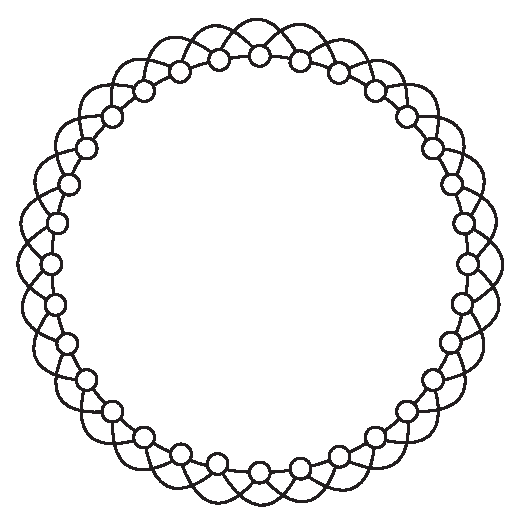
\includegraphics[width=\textwidth]{chapters/02_problem_definition/lattice}
          \captionof{figure}{A lattice.}
          \label{fig:lattice}
        \end{minipage}
        \quad
        \begin{minipage}[b]{0.48\textwidth}
          \centering
          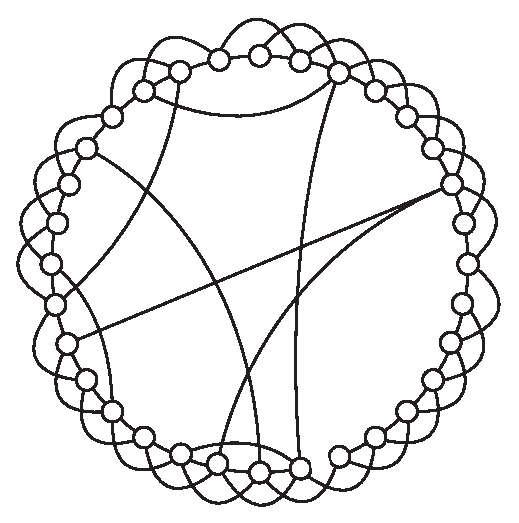
\includegraphics[width=\textwidth]{chapters/02_problem_definition/smallworld}
          \captionof{figure}{A small world model.}
          \label{fig:smallworld}
        \end{minipage}
      \end{figure}

    A certain category of small-world networks were identified as a class of random graphs by Duncan Watts and Steven Strogatz\cite{WattsStrogatz1998}. They noted that graphs could be classified according to two independent structural features, namely the clustering coefficient, and an average shortest path length. Purely random graphs, built according to the Erdős–Rényi (ER) model, exhibit a small average shortest path length (varying typically as the logarithm of the number of nodes) along with a small clustering coefficient\cite{ErdosRenyi1960}. Watts and Strogatz measured that in fact many real-world networks have a small average shortest path length, but also a clustering coefficient significantly higher than expected by random chance. Watts and Strogatz then proposed a novel graph model, currently named the Watts and Strogatz model, with a small average shortest path length, and a large clustering coefficient. The crossover in the Watts-Strogatz model between a \emph{large world} (such as a lattice, see figure \ref{fig:lattice}) and a small world (see figure \ref{fig:smallworld}) was first described by Barthelemy and Amaral in 1999\cite{BarthelemyAmaral1999}.
    
  \section{Network properties}
  
    \subsection{Average path length}
    
      The concept of \emph{average path length} in network topology is that it is the average number of steps along the shortest paths for all possible pairs of vertices in the network. In short, it is a good measure of the efficiency of the network and tells a lot about how quickly the information may be passed over the network. It is one of the three most robust measures of network topology, together with network's clustering coefficient and degree distribution of vertices. The average path length will for example tell how many people one would need to communicate through (on average) to contact a complete stranger. Average path length should not be confused with network diameter, which is the longest geodesic---the longest shortest path between any two nodes in the network.

      With the help of an average path length one can easily tell whether a network is efficient or not. Shorter average path lengths are generally more desirable. However, the average path length only tells what the path length between two nodes will most likely be, as the network itself might have some very remotely connected nodes and many nodes which are neighbours of each other at the same time.
      
      Considering an unweighted graph $G$ with the set of vertices $V$, let $d(v_1, v_2)$, where $v_1, v_2 \in V$ denote the shortest distance between vertices $v_1$ and $v_2$. Assuming that $d(v_1, v_2) = 0$ if $v_1 = v_2$ or if $v_2$ is unreachable from $v_1$. We define the average path length $l_G$ as:
      \begin{equation}
        l_G = \frac{1}{|V| (|V| - 1)} \sum_{i, j} d(v_i, v_j) \mbox{,}
      \end{equation}
      where $|V|$ is the number of vertices in $G$.
      
      In a real world networks like the World Wide Web, a short average path length aids transferring the information quickly and efficiently and also reduces costs. Similarly, by judging average path length of a metabolic network one can tell the efficiency of mass transfer in it. Also, it is possible to minimise a power grid network losses if one can lower the average path length of the network.

      Most real world networks have an average path length which is very short. It leads to a conclusion that a small worlds may exist in such networks and that everyone is connected to everyone else through a very short path. A result being that today, most models of real networks are created with this condition in mind. Several models had been proposed (random network, Watts-Strogatz model, Barabási-Albert model), with all having one thing in common---they all predicted very short average path length\cite{BarabasiAlbert2002}.

      The average path length depends on the system size but does not change drastically with it. Small world network theory predicts that the average path length changes proportionally to $\mbox{log} |V|$, where $|V|$ is the number of nodes in the network.

    \subsection{Transitivity and clustering coefficient}

      In networks it is quite common to find that if vertex A is connected to vertex B and vertex B is connected to vertex C, then the probability that vertex A is connected to vertex C is higher than the probability that vertex A is connected to any other randomly chosen vertex. For example, in social networks, the friends of your friends are more likely to also be your friends than a random person that is not a friend of your friend. This deviation from the behaviour of random graphs can be seen in a network property called \emph{transitivity} (also known as \emph{clustering}, although this term has another meaning which may be confusing). From topological point of view, transitivity means that there are more sets of three vertices, each of which is connected to the other two---called triangles. It may be quantified by defining a \emph{clustering coefficient}
      \begin{equation}
        C = \frac{3 \times \mbox{number of triangles in the network}}{\mbox{number of connected triples of vertices}} = \frac{\mbox{number of closed triplets}}{\mbox{number of connected triples}} \mbox{,}
      \end{equation}
      where a \emph{connected triple} means a single vertex with edges running to an unordered pair of others.

      In graph theory, a clustering coefficient is a measure of degree to which nodes in a graph tend to cluster together. Evidence suggests that in most real-world networks, and in particular social networks, nodes tend to create tightly knit groups characterised by a relatively high density of ties; this likelihood tends to be greater than the average probability of a tie randomly established between two nodes\cite{HollandLeinhardt1971,WattsStrogatz1998}.

      Two versions of this measure exist: the global and the local. The global version was designed to give an overall indication of the clustering in the network, whereas the local gives an indication of the embeddedness of single nodes.

      \subsubsection{Global clustering coefficient}

        The \emph{global clustering coefficient} is based on node triplets. A \emph{node triplet} is made out of three nodes that are joined by either two or three undirected edges, called open and closed triplet respectively. A triangle is built using three closed triplets, one centred on each of the nodes. We define the global clustering coefficient as the number of closed triplets divided by the total number of triplets. Luce and Perry were the first to attempt to measure this quantity\cite{LucePerry1949}. It can be applied to both undirected and directed networks and it gives an indication of the clustering in the whole network. The measure is also called transitivity\cite{WassermanFaust1994}. Watts and Strogatz proposed a following clustering coefficient definition: \textquote{Suppose that a vertex $v$ has $k_v$ neighbours; then at most $k_v(k_v - 1)/2$ edges can exist between them (this occurs when every neighbour of $v$ is connected to every other neighbour of $v$). Let $C_v$ denote the fraction of these allowable edges that actually exist. Define $C$ as the average of $C_v$ over all $v$.}\cite{WattsStrogatz1998}

      \subsubsection{Local clustering coefficient}

        The \emph{local clustering coefficient} of a vertex in a graph assess how close its neighbours are to being a complete graph. The measure was first introduced by Watts and Strogatz to determine whether a graph is a small-world network\cite{WattsStrogatz1998}.

        The neighbourhood $N_i$ for a vertex $v_i$ is defined as its immediately connected neighbours
        \begin{equation}
          N_i = \left\{v_j: e_{ij} \in E \wedge e_{ji} \in E\right\} \mbox{,}
        \end{equation}
        where $e_{ij}$ is an edge connecting vertices $v_i$ and $v_j$.
        
        We define $k_i$ as the number of vertices $|N_i|$ in the neighbourhood $N_i$ of a vertex.

        The local clustering coefficient $C_i$ of a vertex $v_i$ is given by the number of connections within the vertex neighbourhood over the number of connections that could possibly exist between them. Edges $e_{ij}$ and $e_{ji}$ in undirected graphs are considered identical, therefore if a vertex $v_i$ has $k_i$ neighbours, $\frac{k_i(k_i-1)}{2}$ edges could exist among the vertices within the neighbourhood. Hence, we define the local clustering coefficient for undirected graphs as
        \begin{equation}
          C_i = \frac{2\|\{e_{jk}: v_j,v_k \in N_i, e_{jk} \in E\}\|}{k_i(k_i-1)} \mbox{.}
        \end{equation}

        The clustering coefficient can also be defined as
        \begin{equation}
          C_i = \frac{\lambda_G(v)}{\tau_G(v)} \mbox{,}
        \end{equation}
        where $\lambda_G(v)$ is the number of triangles of $v \in V(G)$ (the number of subgraphs of $G$ with 3 edges and 3 vertices, one of which is $v$) and $\tau_G(v)$ is the number of triples on $v \in G$ (the number of subgraphs with 2 edges and 3 vertices, one of which is $v$ and such that $v$ is incident to both edges).

        To show that these two definitions are the same we show that
        \begin{equation}
          \tau_G(v) = C({k_i},2) = \frac{1}{2}k_i(k_i-1) \mbox{.}
        \end{equation}

        The value of the clustering coefficient is within $0$ and $1$ range with the former if no vertex that is connected to $v_i$ connects to any other vertex that is connected to $v_i$ and the latter if every neighbour connected to $v_i$ is also connected to every other vertex within the neighbourhood.

    \subsection{Betweenness centrality}

      Betweenness centrality measures a centrality of a vertex in a network. It is equal to the number of shortest paths from all vertices to all others that pass through that node. Betweenness centrality is one of the most useful measures. It quantifies both the load and importance of a node. Development of this measure is attributed to sociologist Linton Freeman\cite{Freeman1977}.

      The betweenness centrality of a node $v$ is defined as
      \begin{equation}
        g(v) = \sum_{s \neq v \neq t} \frac{\sigma_{st}(v)}{\sigma_{st}} \mbox{,}
      \end{equation}
      where $\sigma_{st}$ is the total number of shortest paths from node $s$ to node $t$ and $\sigma_{st}(v)$ is the number of those paths that pass through $v$.

    \subsection{Degree distribution}

      The \emph{degree distribution} is the probability distribution of degrees of vertices over the whole network. It is defined to be the fraction of nodes in the network with degree $k$
      \begin{equation}
        P(k) = \frac{|V|_k}{|V|} \mbox{,}
      \end{equation}
      where $|V|$ is the number of vertices in a network and $|V|_k$ is the number of vertices in a network having a degree $k$.

      The degree distribution is very important in studying both real networks (such as the Internet and social networks) and theoretical networks. Most networks in the real world have degree distributions that are highly right-skewed, meaning that a large majority of nodes have low degree but a small number, known as \emph{hubs}, have high degree. Some networks, notably the Internet, the World Wide Web, and some social networks are found to have degree distributions that approximately follow a power law
      \begin{equation}
        P(k) \sim k^{−\gamma} \mbox{,} \label{eqn:power_law}
      \end{equation}
      where $\gamma$ is a constant called power law exponent. Networks like that are called scale-free networks and have attracted particular attention for their structural and dynamical properties.
      
      \subsubsection{Scale-free networks}
  
        A scale-free network is a network whose degree distribution follows a power law, at least asymptotically, as defined in equation \ref{eqn:power_law}.
        The power law exponent $\gamma$ is a parameter whose value is typically in the range $2 < \gamma < 3$ for real world networks, although occasionally it may lie outside these bounds\cite{OnnelaSaramakiBarabasi2007,ChoromanskiMatuszakMiekisz2013}.

        Many networks are believed to be scale-free, including the World Wide Web and social networks, although the matter is still under discussion by scientific community as more sophisticated data analysis techniques become available\cite{ClausetShaliziNewman2007}.
        
      \subsubsection{Maximum degree}
      
        The maximum degree $k_{\mbox{max}}$ of a vertex in a network generally depends on the size of the network itself. For some calculations on networks the value of this maximum degree matters. Given a particular degree distribution, the probability of there being exactly $m$ vertices of degree $k$ and no vertices of higher degree is $\binom{n}{m} p^m_k (1 − P_k)^{n−m}$, where $P_k$ is the cumulative probability distribution. Hence, the probability $h_k$ that the highest degree on the graph is $k$ is
        \begin{equation}
          h_k = \sum_{m=1}^n \binom{n}{m} p^m_k (1 - P_k)^{n-m} = (p_k + 1 - P_k)^n - (1 - P_k)^n\mbox{,}
        \end{equation}
        and the expected value of the highest degree is $k_{\mbox{max}} = \sum_k kh_k$.